\section{Methods}  \label{Methods}

In this section We propose a novel RNN architecture called the Recurrent Perceiver to model an object's changing appearance and motion over time for video object detection.

\subsection{Model} \label{Methods:Model}

We build our model architecture based on the Perceiver architecture \cite{jaeglePerceiverGeneralPerception2021}. As discussed in \ref{Background:Perceiver} perceiver has capability of processing high dimantional input which is important for ADS. However, has a limitation of producing only one output per input, which makes it not approapriate for video object detection tasks. To overcome this limitation, we decided to rethink the Perceiver architecture and think of it as a recurrent neural network (RNN) that is capable to process a high dimentional input potentially from different modalities. Hence we have designed a Recurrent Perceiver or RPerciever for short. We have unrolled preceiver in time or in other words we have added a time dinemtion. If previously, the Perceiver was unrolled in depth, we closed the loop and unrolled it in time by propagating the latent array between time steps. For the initial timestamp we still use learnable latent array, the same way it is done in the Perceiver \ref{Background:Perceiver}. The architecture of the perceiver is Figure \ref{fig:figure_methods_model_ar_perceiver}.

% TODO add information about dimentions

% TODO edit fiture and name

\begin{figure}
    \centering
    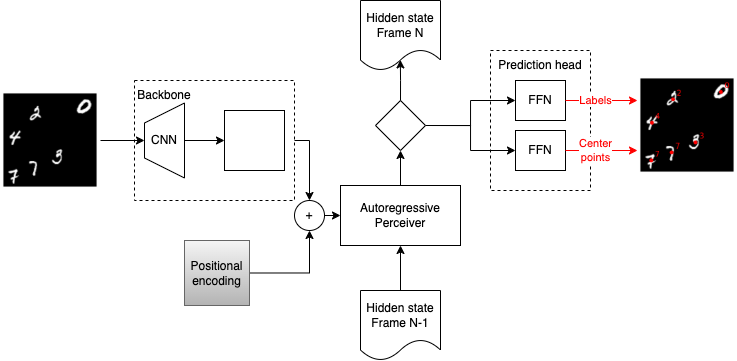
\includegraphics[width=\textwidth]{figures/figure_methods_model_ar_perceiver.png}
    \caption{The autoregressive Perceiver uses a conventional CNN backbone to learn a 2D representation of an input frame. The model flattens it and supplements it with a positional encoding before passing it to the autoregressive Perceiver model. Additionally, the autoregressive Perceiver takes a hidden state from the previous frame. We pass each output embedding of the Perceiver to the feed-forward network (FFN) that predicts class labels and center points.}
    \label{fig:figure_methods_model_ar_perceiver}
\end{figure}

We designed a variation of the RPerceiver to process multi-modal input. We call this arcitecture as Recurrent Perceiver Multi-Modal or RPerceiverMM for short. Modern ADS process information from multiple sensors. In the scope of the thesis, we consider a multi-view camera setup. \cite{jaeglePerceiverGeneralPerception2021} consider a multi-modality input where modality specific by concatenating a learned, modality-specific encoding to each input. In our work we followed a different approach for multi-modality. ADS is equiped with multiple cameras that are placed in different locations. There's exists a problem of calibrating. Therefore we decided to intorduce a camera specific cross-attention module to the RPerceiverMM. The architecture of the RPerceiverMM is shown on Figure~\ref{fig:figure_methods_model_ar_perceiver_views}.

% TODO edit fiture and name

\begin{figure}
    \centering
    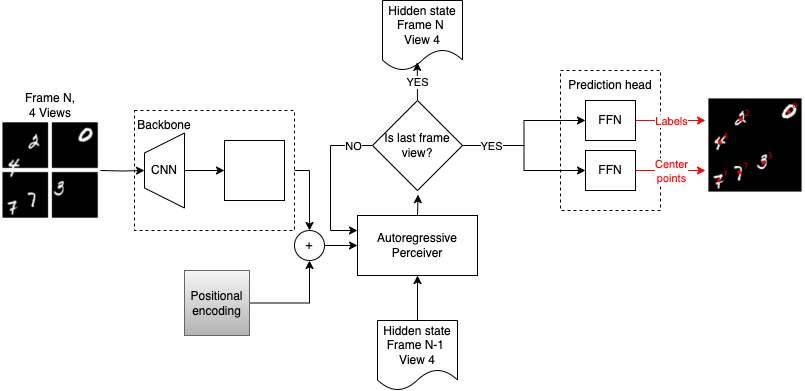
\includegraphics[width=\textwidth]{figures/figure_methods_model_ar_perceiver_views.png}
    \caption{Autoregressive Perceiver with view dimension. The backbone output is supplemented with a learned view-specific positional encoding before passing it to the autoregressive Perceiver model. The autoregressive Perceiver takes a hidden state from the previous frame's last view and iterates through the current frame's views. After the last view, we pass the output embedding of the Perceiver to the feed-forward network (FFN) that predicts class labels and center points on the global frame raster.}
    \label{fig:figure_methods_model_ar_perceiver_views}
\end{figure}

Additionally, to the Recurrent Perceiver (including Multi-modal variant), we used a CNN backbone to learn a 2D representation of the input frames, we did not use a pre-trained backbone see Appendix \ref{Appendix:Backbone}. We used a detection heads similar as in DETR model \cite{} with linear layer to project class logits and 3 layer of multi-layer perceptron (MLP) to predict the object coordinates. As for objects coordinates we considered two variants: (i) bounding boxes (ii) center point. Therefore the dimention of output $Lx4$ and $Lx2$ respectively. For bounding boxes we used a sigmoid activateion function to predict coordinates of bounding box center and width and hight. For center points we used a tanh activation function because we placed the center of the coordnate system into the center in order to mimic a berd-eye view, similar as ADS in center with all views around it. The whole and complete architecture is show \ref{fig:figure_methods_model_r_perceiver_complte}.

\begin{figure}
    \centering
    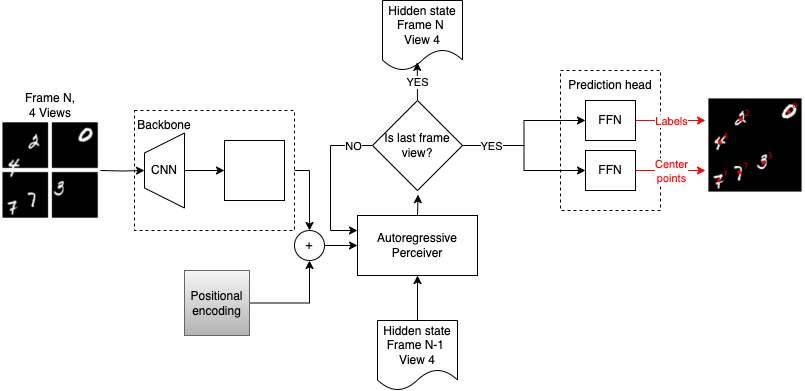
\includegraphics[width=\textwidth]{figures/figure_methods_model_ar_perceiver_views.png}
    \caption{Full architecture of our model. The backbone output is supplemented with a learned view-specific positional encoding before passing it to the autoregressive Perceiver model. The autoregressive Perceiver takes a hidden state from the previous frame's last view and iterates through the current frame's views. After the last view, we pass the output embedding of the Perceiver to the feed-forward network (FFN) that predicts class labels and center points on the global frame raster.}
    \label{fig:figure_methods_model_r_perceiver_complte}
\end{figure}


\subsection{Dataset} \label{Methods:Dataset}

For our experiment, we generated our own dataset, which we call "detection-moving-mnist-easy". We took inspiration from the MovingMNIST dataset \cite{srivastava2016unsupervisedlearningvideorepresentations}, which is used for TODO use cases. In our case, we are interested in video object detection and a simplified variation of keypoints, where we predict a center point of the object it is similar to keypoints task because the center of object is not the same as center of the bounding box. We hosted the dataset on Hugging Face \footnote{\url{https://huggingface.co/datasets/Max-Ploter/detection-moving-mnist-easy}}.

 For the first frame, we pick a number of digits from 1 to 10 with uniform probability (see Figure~\ref{fig:figure_method_dataset_train_digit_classes}). Depending on the number of digits per first frame, we draw, without replacement, from the well-known MNIST dataset \cite{} (from the train and test splits corresponding to the dataset split). Each digit is placed on the first frame of the canvas image of size 128x128. There's a greedy algorithm that places digits on the first frame randomly and tries to avoid overlaps, so it's easier for the model to detect all objects in the beginning. To each digit, we assign an affine translation from -5 to 5 randomly with uniform probability. Then, we apply corresponding affine transformations to move the digits through 20 frames on the canvas image of size 128x128. As a result, we receive a tensor of size 20x1x128x128, which represents a video (see Figure~\ref{fig:figure_methods_dataset_detection_mmnist_sequence}).

\begin{figure}
    \centering
    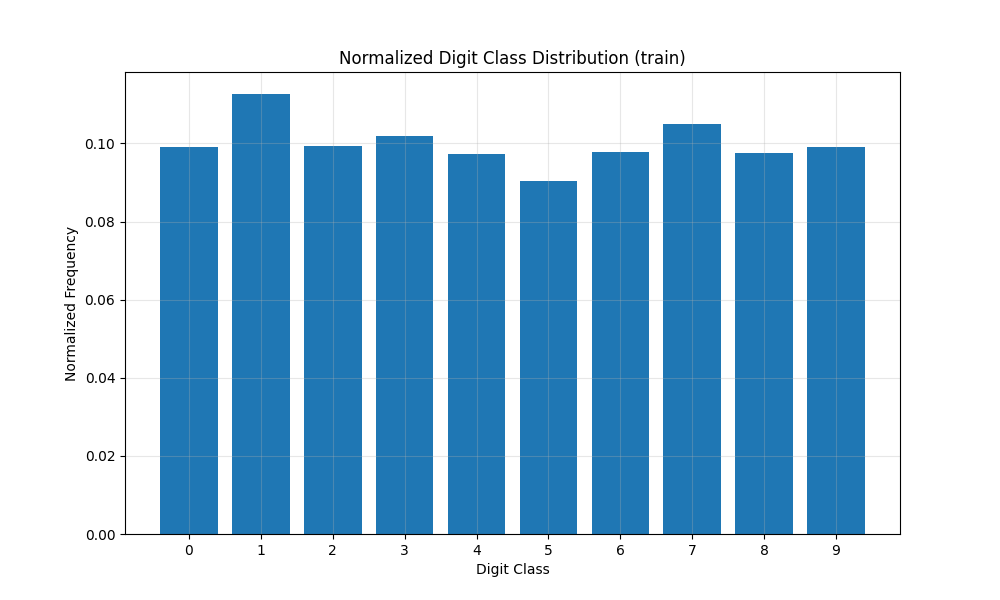
\includegraphics[width=\textwidth]{figures/figure_method_dataset_train_digit_classes.png}
    \caption{Distribution of classes in the "detection-moving-mnist-easy" dataset.}
    \label{fig:figure_method_dataset_train_digit_classes}
\end{figure}


\begin{figure}
    \centering
    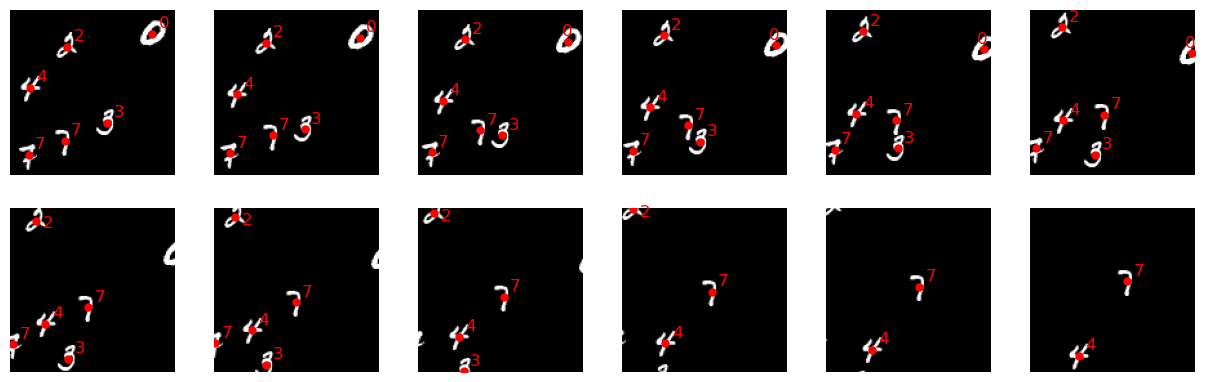
\includegraphics[width=\textwidth]{figures/figure_methods_dataset_detection_mmnist_sequence.png}
    \caption{Example of 12 frames from the sequence. Ground truth, shown in red, indicates the ground truth digit center point and a class label.}
    \label{fig:figure_methods_dataset_detection_mmnist_sequence}
\end{figure}


In order for dataset to be more challanging we do not restrict digit overlap in subsequent frames. It is even possible to have some degree of overlap in the first frame if the greedy algorithm is unable to randomly place digits in such a way on the first frame. We do not bounce digits against image boundaries, so each digit can leave the frame. You can see in the figure that later frames have fewer digits (see Figure~\ref{fig:figure_method_dataset_train_digits_per_frame}).

% TODO DOUBLE CHECK number this plot
\begin{figure}
    \centering
    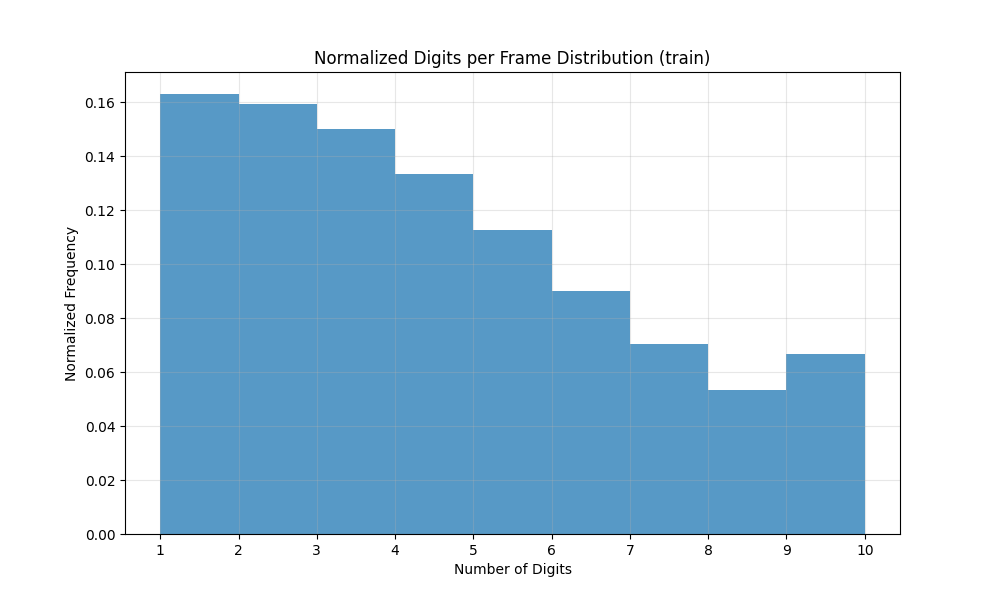
\includegraphics[width=\textwidth]{figures/figure_method_dataset_train_digits_per_frame.png}
    \caption{Distribution of classes in the "detection-moving-mnist-easy" dataset.}
    \label{fig:figure_method_dataset_train_digits_per_frame}
\end{figure}

We generated the dataset with 60K and 10K train and test splits, respectively. Annotations, automatically generated during sequence creation, include digit classes and digit center point coordinates (keypoint), bounding box coordinates and digit's identity ID.

\subsection{Metrics} \label{Methods:Metrics}

We used mean Average Precision (mAP) as the primary metric to evaluate the model's performance. A widely used metric in object detection, mAP measures the average precision across various Intersection over Union (IoU) thresholds, adapted from information retrieval evaluation methods and popularized in challenges like PASCAL VOC \cite{everinghamPascalVisualObject2010}. Specifically, we report the mAP at an IoU threshold of 0.5, a common choice established in early object detection benchmarks such as PASCAL VOC \cite{everinghamPascalVisualObject2010}, and the mAP at 0.5-0.95, which represents the mean of the average precision calculated at IoU thresholds ranging from 0.5 to 0.95 with a step of 0.05, as introduced by the COCO challenge \cite{linMicrosoftCOCOCommon2015a}.

We used the Average Displacement Error (ADE) and Final Displacement Error (FDE) metrics to evaluate the model's performance. The ADE measures the average distance between the predicted and ground truth center points over the sequence of frames \ref{eq:ade}.

\begin{equation}
    \text{ADE} = \frac{1}{N \cdot T} \sum_{i=1}^{N} \sum_{t=1}^{T} || \hat{y}_{i,t} - y_{i,t} ||_2
    \label{eq:ade}
\end{equation}

The FDE measures the distance between the predicted and ground truth center points at the last frame of the sequence \ref{eq:fde}.

\begin{equation}
    \text{FDE} = \frac{1}{N} \sum_{i=1}^{N} || \hat{y}_{i,T} - y_{i,T} ||_2
    \label{eq:fde}
\end{equation}

\subsection{Training} \label{Methods:Training}

Augment
Loss
Optimizer
reference to all hyperparameters in appendix


\subsection{Dropout and Shuffle} \label{Methods:Training:DropoutAndShuffle}

We implemented two training procedures: \texttt{shuffle} and \texttt{dropout}. Additionally, we implemented a combination of the two. A model trained without applying these training procedures is considered the baseline.

\begin{description}
    \item[\texttt{shuffle}] In this procedure, the sensor inputs are randomly permuted within each time step. Consequently, the model receives inputs from the sensors in a random order for that specific time step. This shuffling only occurs for sensor inputs within the same time step. This training procedure is only applicable to a multi-view setup.

    \item[\texttt{dropout}] This procedure simulates scenarios where sensor information is missing. To achieve this, we train the model by intermittently dropping sensor inputs (input dropout). We keep the first half of the input sequence intact (no dropout), allowing the model to accumulate features in its hidden state. The second half of the sequence may undergo frame dropout depending on the dropout probability. During training, we gradually increase the probability of an information dropout from 10\% up to 86.6\%.
\end{description}



% TODO add schema of shuffle and dropout

% TASK DEFINITION

% METRICS